%\section{Analysis of Europa Moon surface and Environment}
\section{The Radiation Environment}\label{sec:radiation_environment}
Jupiter’s magnetic field, shaped as a toroidal, affects the radiation environment around the planet by interacting with the solar wind trapping energetic particles, creating radiation belts similar to van Allen belts on Earth but with much higher intensity. This magnetosphere of charged particles extends radially from 50 to 100 RJ. For purpose of practicality this area is subdivided into three main regions, the outer magnetosphere ($>$40 RJ), middle (10-40 RJ) and the inner magnetosphere ($<$10 RJ). For our purpose, we are focusing on the middle region, an area where Europa lays along with the rest of the four Galilean moons, Io, Ganymede and Calisto. Highly energetic charged particles are trapped within that region, mainly electrons and protons but also ions, ranging from a few keV up to tens of MeV. Here we can also locate the Io plasma torus, created by the interaction of the rotating magnetic field of Jupiter with the spewed volcanic gasses of Io, drifting and ionizing them into plasma.

Axial tilt of the magnetic dipole of Jupiter and consequently of the spin plane, causes Europa to cruise in and out of the plane by 10$^circ$ north and south of the magnetic latitude affecting the radiation environment of the moon. 

Through a process known as sputtering, bombardment of Europa’s surface with highly ionizing particles causes the ejection of surface molecules where some of them manage to escape gravitational pull of the moon and get accelerated by the co-rotating magnetosphere creating an additional contribution to the particle distribution. 

Data collected by Galileo, Voyager and Pioneer spacecraft missions show high intensities of energetic particles fluxes around Europa’s orbit area varying in time to a limited extent. Electrons intensity (fig. \ref{electrons energy}) show a wide spectra of energies dominating on that region but with a large variation on lower energies due to the high uncertainty rates of the detectors during these missions and especially from Galileo.
\begin{figure}[htb]
\centering
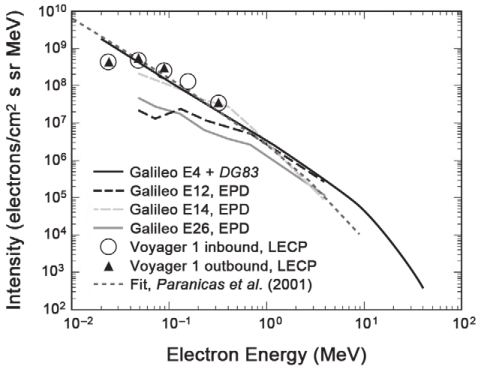
\includegraphics[width=0.5\textwidth]{figures/Orbiter/electrons_energy_spectrum}
\caption{Energy spectrum of electrons near Europa’s orbit from various sources, \cite{paranicas2009europa}.}
\label{electrons energy}
\end{figure}
Several Galileo close encounters to Europa’s orbit, reveal the energy distribution of proton, oxygen and sulfur ions and show high intensities at high energies while on low energies a greater variation between the ions is observed (fig. \ref{fig:ions_energy}).
\begin{figure}[htb]
    \centering
    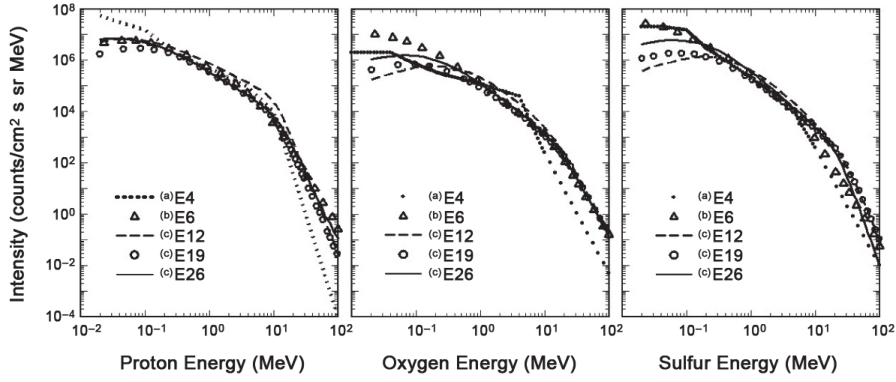
\includegraphics[width=0.80\textwidth]{figures/Orbiter/ions_energy}
    \caption{Ion energy spectra data acquired from Galileo mission on various encounters of Europa at distances of 692 km (E4), 586 km (E6), 201 km (E12), 1439 km (E19), and 351 km (E26) \cite{paranicas2009europa}}
    \label{fig:ions_energy}
\end{figure}
\section{Current Studies of the Surface}\label{sec:surface_studies}
Delivering a lander vehicle on Europa, requires a thorough knowledge of the surface composition and characteristics. On a large scale the surface looks smooth and without great variations but on a higher spatial resolution we can notice the complexity of the terrain. Smooth plains, lenticulae and chaos regions dominate the morphology and topography of the moon’s surface. Many models have suggested that formation of these terrain features involves hydrothermal activity within the ice shell causing fractures and ridges (fig\ref{fig:europa_surface}). 
\begin{figure}[htb]
    \centering
    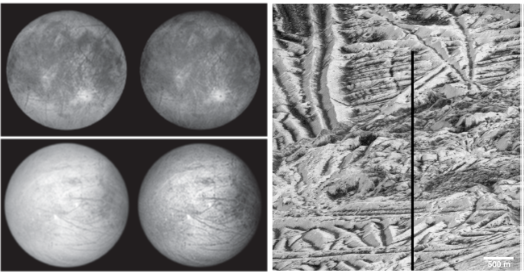
\includegraphics[scale=0.6]{figures/Orbiter/europa_surface.png}
    \caption{Left: Europa’s trailing (top) and leading (bottom) hemispheres as imaged from Galileo on the left and enhanced on the right to illustrate the geological complexity of the surface. Right: A close up look of the surface \cite{carlson2009europa}}
    \label{fig:europa_surface}
\end{figure}
Studies of the surface composition, suggest that Europa was formed by endogenic and exogenic sources of materials. Endogenic sources include either thermochemical reactions that have created hydrated silicates, iron oxides and carbon-nitrogen compounds or unaltered silicates, nickel-iron compounds, organic matter and water, depending on the initial conditions of the protojovian nebula. As for exogenic material, three main sources have been identified. Io’s ejected material reaching Europa by its thermal plasma torus, material outside of the Jovian system delivered by comets and asteroids, and material from the outer Jovian satellites ejected from their surfaces.
%\todo[inline]{Other missions - Galileo et al.}
\section{Lenticulae}\label{sec:lenticulae}
On the surface of Europa a number of circular and elliptical formations are observed, named as lenticulae (fig. \ref{fig:lenticulae}). Many of these are domed hills, cavities and others seems to be dark and flat blemishes. Some appear to have a rough surface with a chaotic structure. The peaks of these domes, show similarities with the composition of the nearby surface, indicating that they have been probably created when the crust forced from below due to some geological events, similar to the magma chambers on Earth. Origin of the flat dark blemishes seems to be melted ice that has been released from cracks of the surface.
\begin{figure}[htb]
    \centering
    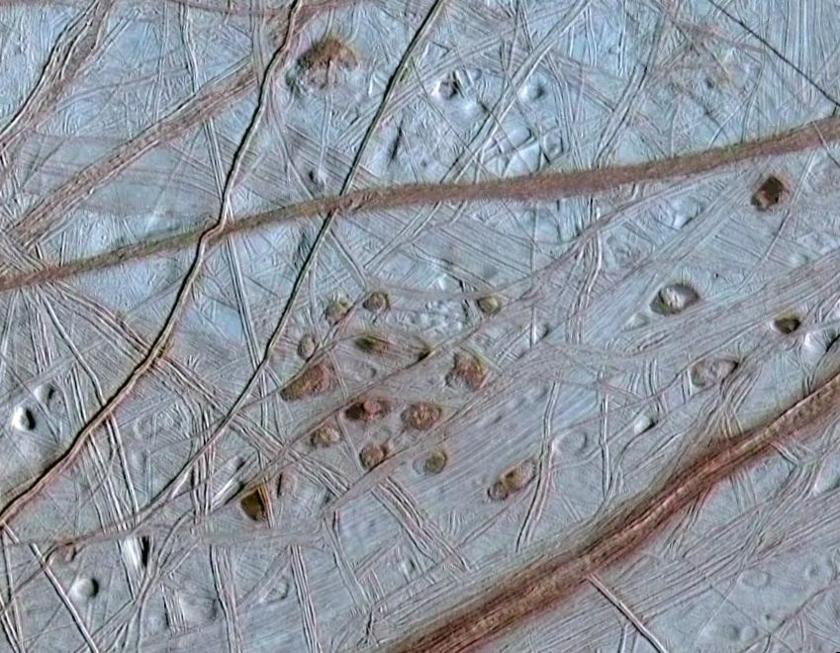
\includegraphics[scale=0.3]{figures/Orbiter/lenticulae.jpg}
    \caption{Lenticulae on Europa's surface / Courtesy of Galileo Project, NASA}
    \label{fig:lenticulae}
\end{figure}
\section{Chaos regions}
About one quarter of Europa’s surface is covered by highly disrupted areas mostly known as chaotic regions.  Most of these chaotic regions are concentrated in two oval shaped areas within 40$^{\circ}$ of the equator and centred at 120$^{\circ}$ and 300$^{\circ}$ W probably because these areas correspond to the location of paleopoles before the reorientation event, where tidal heating is more active. Also regions like Thera Macula, a low lying area with possible subsurface water, provide an indication of present active chaotic formation. Morphologically, chaos regions can vary presenting distinct characteristics or even combinations of them.

Plates of preexisting terrain are characterised by a spanning between 1-20km across, usually elevated from the surrounding area or with one of their edges tilted. Reconstruction models have shown that most of these plates have moved from their original positions, with 22\% of them showing a movement of over 5km. Other areas present inward facing scarps, slopes extending upwards into their neighbour terrain or even signs of chaotic terrain flowing into nearby ridges.
Numerous existing models have tried to describe the geophysical process of formation of these regions with the melting through the icy shell and brine mobilization models being the predominant, managing to explain most of the key and secondary observations. Melting through the icy shell model suggests that heat originating from the seafloor manages to melt the ice crust creating pits beneath the surface ice, while brine mobilization includes materials with low melting point conducting heat within the ice, lowering its viscosity and allowing leakage of liquids through the shell. Other models propose exogenic impacts on the surface as a mechanism of chaos region creation, while rising diapirs may be used to explain some large dome features.  
\begin{figure}[htb]
    \centering
    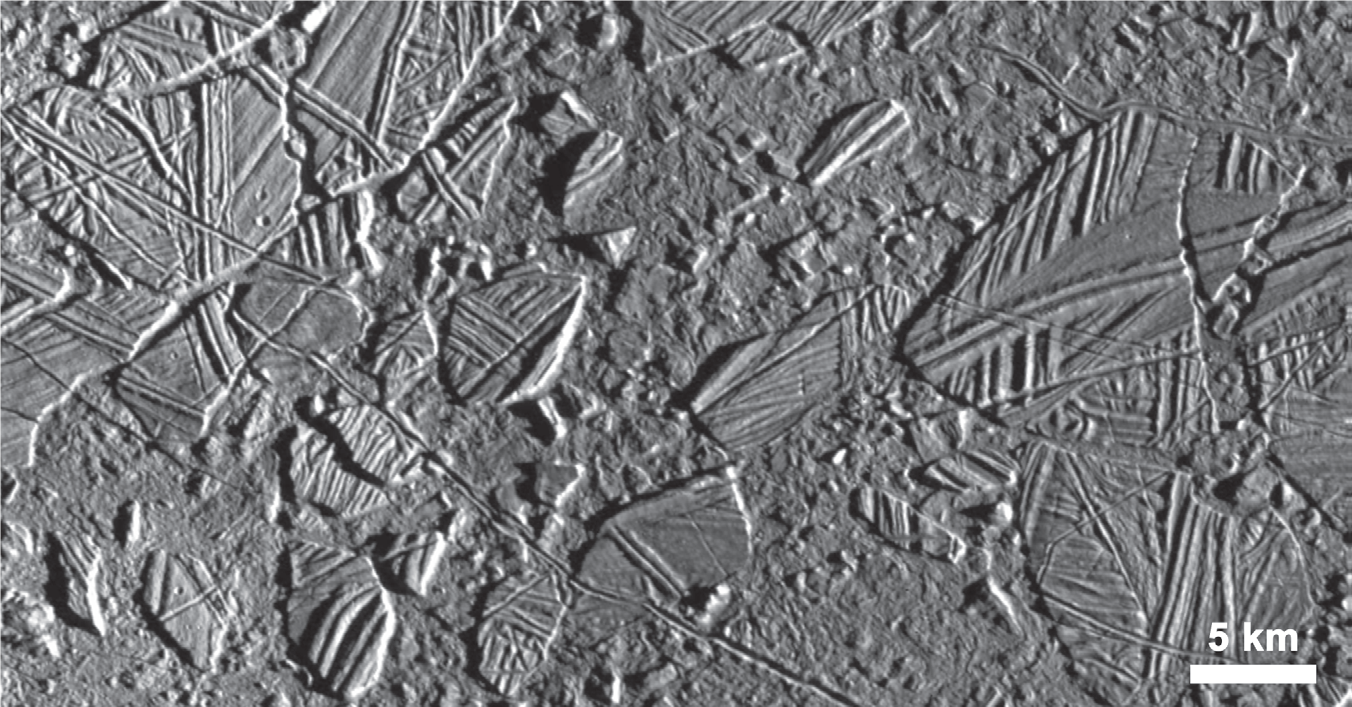
\includegraphics[scale=0.3]{figures/Orbiter/chaos.png}
    \caption{Conamara Chaos, Galileo E6ESBRTPLN01 observation \cite{chaosterrain}}
    \label{fig:conamara_chaos}
\end{figure}
Something that characterize the surface of these regions, is their distinctive dark red-brown color. Origin and exact composition of the material present on these area is still under investigation since not enough data are available but some estimations predict that probably is originating from sulfur compounds produced via radiolysis on the surface. Additionally spectral analysis of the same region on the infrared spectra, indicates the presence of a hydrated material like sulfate salts or sulfuric acid hydrate. If this estimation is confirmed then the low melting point of these materials, compared to the one of pure water ice, adds an important aspect in the formation of the chaos regions.
\begin{itemize}
    \item Avoid certain areas (brown areas, chemical compositions)
\end{itemize}
\todo[inline]{Resolution provided by current imaging from casini and imaging spectrometers?}
\todo[inline]{Is 30 percent a realistic coverage? Why? Give a rough estimate of the suitable landing zones. }

